\newcounter{nonstaggeredpauses}
\newcounter{staggeredpauses}

\begin{frame}
\frametitle{Finite Volume Method (FVM)}
\begin{columns}[c]

\column{.6\textwidth}
\begin{itemize}[<+(1)->]
\item The space is divided into a finite number of volume elements
\item Properties are stored on discretized points in the cells
\setcounter{nonstaggeredpauses}{\thebeamerpauses}
\item Vector fields can sometimes be discretized to cell faces (known as \emph{staggered grid})
\setcounter{staggeredpauses}{\thebeamerpauses}
%\let\b\thebeamerpauses
\end{itemize}

\column{.45\textwidth}

\begin{figure}
\centering
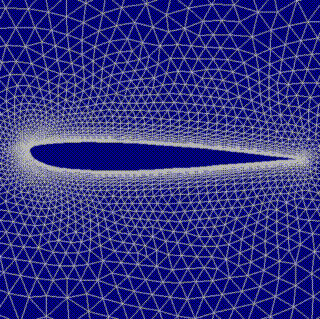
\includegraphics[width=.5\textwidth]{Images/Attribute/Grid/Zhukovskii_profile_by_NASA}
\caption{Retrieved from commons.wikimedia.org/wiki/\allowbreak File:Zhukovskii\_profile\_by\_NASA.gif}
%\allowbreak 
%\end{figure}
%\begin{figure}
%\centering
\uncover<\thenonstaggeredpauses->{
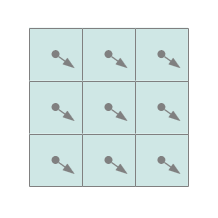
\includegraphics[width=0.35\textwidth]{Images/Attribute/Staggered/Staggered_grid_schema1}
\quad
\uncover<\thestaggeredpauses->{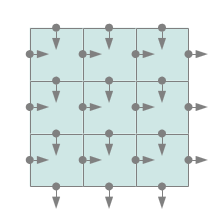
\includegraphics[width=0.35\textwidth]{Images/Attribute/Staggered/Staggered_grid_schema2}}
\caption{Retrieved from http://commons.wikimedia.org/\allowbreak wiki/File:Staggered\_grid\_schema.png}
}
%\allowbreak 
\end{figure}

\end{columns}
\end{frame}